\section{Solipsis}
	\label{solipsis}
	Solipsis est le "socle" du travail Blue Banana, nous allons le présenter rapidement et voir les propriétés importantes qui caractérisent Solipsis.
	\subsection{Introduction sur Solipsis} 
	\par Nous allons expliquer le fonctionnement global et les fonctionnalités importantes de Solipsis. Solipsis est fait pour accepter un nombre illimité d'utilisateurs et pour maintenir une cohérence suffisante . Il peut être accessible par n'importe quel ordinateur, il peut fonctionner sur des ordinateurs peu puissants et avec des connections internet faibles (56Kbs) ou sans fil. Une fois les nœuds connectés, ils peuvent échanger des données telles que de la vidéo, du son, le mouvement d'avatar ou toutes choses affectant la représentation du monde virtuel. \\
	\subsection{Propriétés de Solipsis}
	Le monde de Solipsis est un tore à deux dimensions, chaque entité détermine sa position dans le monde et elle en est responsable. Chaque utilisateur collecte les informations lui permettant de reconstituer son environnement virtuel local. Les connections entre les nœuds sont bidirectionnelles. 
		\subsubsection{Propriétés}
	Solipsis doit permettre aux utilisateurs de se déplacer à travers le monde, il faut pour cela que les deux propriétés locales suivantes soient respectées.
	\begin{itemize}
	\renewcommand{\labelitemi}{$\bullet$}
		\item \textit{Local Awareness:}\\
		Une entité doit être connecté avec tous ses plus proches voisins. Il est important de noter qu'une entité a la possibilité de connaître des entités en dehors de son environnement virtuel local. En revanche, cette propriété impose que l'entité situé à l'intérieur.	
		\item \textit{Global Connectivity:}\\
		Une entité doit connaître toutes les entités se trouvant dans son "champs de vision". Elle doit pouvoir détecter l'arrivée ou le départ d'un entité de son "champs de vision". Cette propriété est basée sur la Géométrie Informatique, elle assure qu'une entité ne "tourne pas le dos" à une partie du monde. L'enveloppe convexe des entités est le plus petit polygone convexe formé par cet ensemble. Un mécanisme pour éviter qu'une partie du graphe soit isolée a aussi été mis en place.\\
	\end{itemize}
        \vspace{1cm}
	\begin{figure}[!h]
	\centering
        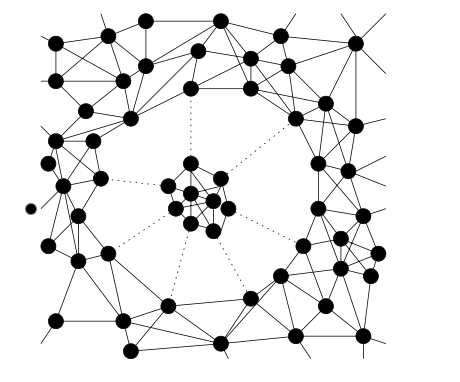
\includegraphics[scale=0.9]{../Images/composant_isole1.png}\\
        \caption{Un composant connexe isolé et les connexions qui évitent la création d'une île}
        \label{Envelop_Convex}
        \end{figure}

		\subsubsection{Maintien des propriétés}
Solipsis a aussi des mécanismes de collaboration pour maintenir les propriétés précédentes, nous allons voir ces deux propriétés:
	\begin{itemize}
	\renewcommand{\labelitemi}{$\bullet$}
		\item \textit{Spontaneous Collaboration for Local Awareness:}\\
		 Pour vérifier la propriété \textit{Local Awareness}, il faut qu'une entité puisse connaître tous ses voisins à chaque instant. Pour faciliter cette connaissance du voisinage, et comme il y a un grand nombre de mouvements dans le monde virtuel, un système de collaboration entre les nœuds a été mis en place. Une entité pourra alors demander régulièrement à ses voisins si ils détectent une nouvelle entité mais cela implique un grand nombre de message inutile et une perte temporelle de consistence. Pour éviter ces problèmes, une entité \textit{a} va prévenir une entité \textit{b} si une entité \textit{c} est en train de se diriger vers la zone de l'entité \textit{b}.
		\item \textit{Recursive Query-Response for Global Connectivity:}\\
		Il faut prévoir une mécanisme pour le maintien d'une entité dans l'enveloppe convexe. Quand une entité \textit{e} détecte deux entités consécutives, elle se lance immédiatement à la recherche d'une ou plusieurs entités dans le même secteur en envoyant des messages dans la zone. \\ 
	\end{itemize}
        \vspace{1cm}
        \begin{figure}[!h]
	\centering
        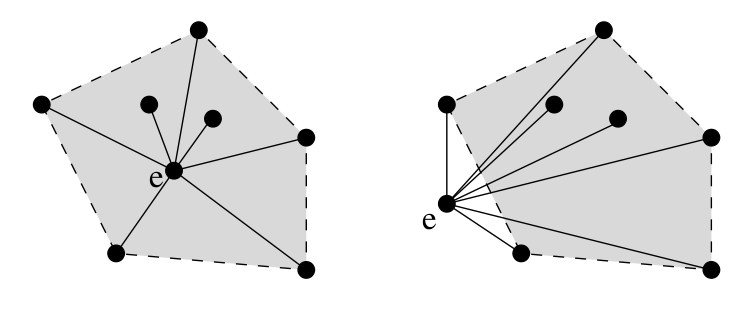
\includegraphics[scale=0.9]{../Images/envelop_convex1.png}\\
        \caption{Deux différentes enveloppes convexes des voisins de \textit{e}. A gauche, \textit{e} respecte la règle de \textit{Global Connectivity} et à droite non.}
        \label{Envelop_Convex}
        \end{figure}
